% The most comprehensible way of showing your final design 
% (and why it matters) is to give a walkthrough of the key task.
%
% make a sequence of screenshots. Crop and add callouts if necessary 
% to reveal detail such as text in the UI.
%
% Start by showing the final design, then explain why you did it
% 
% keep intro and walkthrough short by explaining only 
% (this is not literature class. Don’t give in to “but if I say 
% everything right away, why would attendees/readers continue to 
% pay attention?”
%
\clearpage
\subsection{Walkthrough - Photo Browsing}
%
As we found out during User Studies and the Contextual Inquiry, one of the most widely used features of social websites is picture browsing.
That is why we provide corresponding functionality to perform this task.

\begin{figure}[h]
  \begin{center}
    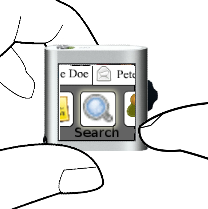
\includegraphics[width=0.6\linewidth]{imgs/wt1.png}
  \end{center}
  \caption{The Main Screen with Vertical Scrolling, Thumb-sized Icons}
  \label{fig:wt1}
\end{figure}
%
As shown in Fig. \ref{fig:wt1}, every action performed by a user starts in the Main Menu. There is a ticker on top of it, covering the latest news from your friends. Scrolling through the menu is done by swiping gestures or the thumbwheel.
To browse the pictures of a person, we have to find the person first. That is why the search function is selected, simply by tapping on the icon.

\begin{figure}[h]
  \begin{center}
    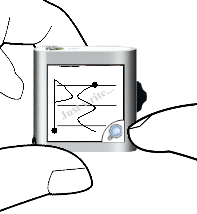
\includegraphics[width=0.6\linewidth]{imgs/wt2.png}
  \end{center}
  \caption{The Writing Recognition Offers Visual Feedback}
  \label{fig:wt2}
\end{figure}
%
To proceed, the name of the person is typed in, as shown in Fig. \ref{fig:wt2}.
\\
\begin{figure}[h]
  \begin{center}
    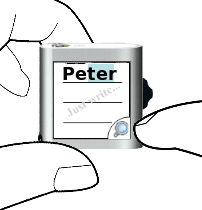
\includegraphics[width=0.6\linewidth]{imgs/wt3.png}
  \end{center}
  \caption{Type-Ahead for Quick Access}
  \label{fig:wt3}
\end{figure}
%
Auto-completion features are used to provide easier and effortless text input (Fig. \ref{fig:wt3}) which is crucial on very small screens.\\
\begin{figure}[h]
  \begin{center}
    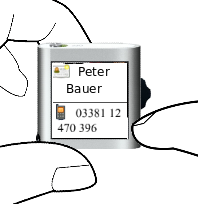
\includegraphics[width=0.6\linewidth]{imgs/wt4.png}
  \end{center}
  \caption{A Vertically Scrolling Profile View}
  \label{fig:wt4}
\end{figure}
%
The Profile View on our device, as depicted in Fig. \ref{fig:wt4}, shows a set of the most important information on the respective person. Again, scrolling through the menu is done by gestures or the thumbwheel.\\
%
\begin{figure}[h!]
  \begin{center}
    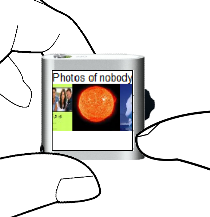
\includegraphics[width=0.6\linewidth]{imgs/wt5.png}
  \end{center}
  \caption{Viewing Albums of a User}
  \label{fig:wt5}
\end{figure}
%
Concerning interaction, viewing photo albums (Fig. \ref{fig:wt5}) is just the same as browsing the Main Menu. This ensures a consistent look-and-feel throughout our user interface.

\begin{figure}[h]
  \begin{center}
    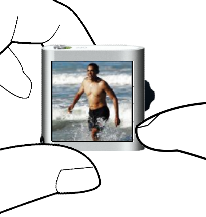
\includegraphics[width=0.6\linewidth]{imgs/wt6.png}
  \end{center}
  \caption{A Fullscreen Photo View}
  \label{fig:wt6}
\end{figure}
%
Concerning the limitations of a Euro-sized screen, we decided that the actual Photo View has to be done in Fullscreen mode, as displayed in Fig. \ref{fig:wt6}. That way, pictures remain recognizable within reasonable distances.
%
